% Nallino, Part I p. 290: Schiaparelli's figure of the apparent diameter of an epicycle, redrawn from the print:
% the epicycle about O, the tangents XA and XB from the eye X, the line XO and the dotted radius OB.
% Measured on the scan (_intake/latin/tools/fig290).
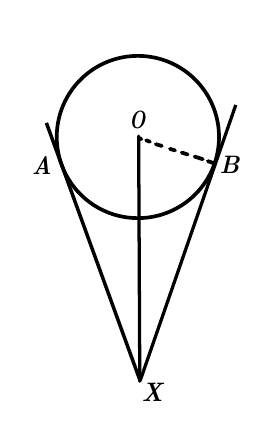
\begin{tikzpicture}[x=0.9864pt,y=-0.9864pt,line cap=butt,every node/.style={font=\fontsize{11}{11}\bfseries\itshape\selectfont,inner sep=0pt}]
\useasboundingbox (0,0) rectangle (80.00,138.50);
\draw[line width=1.33pt] (40.37,40.05) circle[radius=29.72];  % the epicycle about O
\draw[line width=1.26pt] (41.20,129.34) -- (6.86,34.88);  % the tangent XA, from the eye X to the end of its ink above A
\draw[line width=1.18pt] (41.20,129.34) -- (76.23,28.32);  % the tangent XB, from the eye X to the end of its ink above B
% the line XO
\draw[line width=1.18pt,line cap=round] (41.07,129.53)--(40.65,39.71);
% the dotted radius OB, dash by dash
\draw[line width=1.37pt,line cap=round] (40.65,40.49)--(41.65,40.82) (43.41,41.27)--(44.79,41.77) (46.93,42.68)--(49.13,43.32) (52.13,44.41)--(53.99,44.97) (56.41,45.75)--(58.61,46.46) (61.16,47.22)--(64.12,48.17) (66.02,48.90)--(68.78,49.81);
\node at (40.14,33.72) {\normalfont\fontsize{11}{11}\bfseries\itshape\selectfont \resizebox{5.91pt}{6.16pt}{O}};
\node at (5.19,50.76) {\normalfont\fontsize{11}{11}\bfseries\itshape\selectfont \resizebox{7.14pt}{6.25pt}{A}};
\node at (73.92,50.40) {\normalfont\fontsize{11}{11}\bfseries\itshape\selectfont \resizebox{7.19pt}{6.25pt}{B}};
\node at (45.61,133.50) {\normalfont\fontsize{11}{11}\bfseries\itshape\selectfont \resizebox{7.67pt}{6.62pt}{X}};
\end{tikzpicture}
